\chapter{Future Work Recommendations}
\label{chap:future}

This chapter discusses in brief the other problems that have been recognised within the scope of UD. None of these works mentioned in this chapter have been discussed in the present version of the document. For future researchers interested in tackling more problems with respect to UD, this chapter could be a good point of reference. 

\section{Enhanced Dependencies}
\label{future:enhanced}

Enhanced Dependencies can be understood as an additional layer of annotation of dependencies in UD, which essentially marks added dependencies. Considering some of the restrictions imposed by the regular annotation scheme like a singular head constraint where each node can have only one head, the Enhanced Dependencies aim to cover aspects which can be missed by the regular annotation scheme. However, not all of the languages, or their treebanks have been annotated with the Enhanced Dependencies so far. While the enhanced dependencies have been deemed to be useful in multiple cases (like that of ellipsis, cf. Section \ref{future:ellipsis}), their full potential might not have been realized so far.

In our experiment on \verb|conj_head| (cf. Chapter \ref{chap:conj_head}), we did not work with the problem of conjunction sandwiches. It is very likely that such problems which are difficult to be recognized by the regular dependencies can be searched for rather easily with the Enhanced Dependencies. For example, if Enhanced Dependencies mark all the conjuncts by the \texttt{conj} deprel, regardless of whether they are labelled by the deprel in the regular annotation or not, it would allow searching for the available conjuncts rather easily.

We leave it as an open problem for future research to identify cases which are more difficult to handle with regular dependencies, while trying to use Enhanced Dependencies. As an add-on to the task, it can also be tested if some algorithms mentioned in the research can be improved upon or discarded when Enhanced Dependencies are used.

\section{Ellipsis}
\label{future:ellipsis}

The problem with annotation of Elliptical Structures is big enough to warrant a discussion of its own in UD Annotation Guidelines\footnote{\url{https://universaldependencies.org/u/overview/enhanced-syntax.html\#ellipsis}}\textsuperscript{,}\footnote{\url{https://universaldependencies.org/u/overview/specific-syntax.html\#ellipsis}}. 

\cite{orphan} analyzed the elliptical constructions in UDv2.0 treebanks \citep{UDv2.0} by principally using \verb|orphan| relations\footnote{\url{https://universaldependencies.org/u/dep/orphan.html}} as a way to identify the cases of non-promoted dependents with promoted dependents. While this helps in identifying only a certain number of cases, it fails to identify the cases where the dependents are promoted. 

In Enhanced Dependencies, \verb|orphan| is replaced by placing a null node to indicate the elided token. However, as discussed earlier, Enhanced Dependencies are not available for all languages or even all treebanks in the same language. Thus, the identification and correction of erroneous elliptical constructions remains a problem that needs to be solved within the scope of basic dependency graphs in UD.

\section{\texttt{FalseNonProjective}: Introduction of False Non-Projectivity into the Annotation}
\label{future:nonproj}

While non-projectivity is a characteristic of some languages, and especially more so of certain genres (poetry, for example); the increasing count of non-projective trees has been shown to affect dependency parsing in a negative way. Owing to semi-automatic conversion scheme, a lot of non-projectivities might also be introduced artificially. Thus, it becomes important to not only identify such cases of false non-projectivities (i.e. the cases which should have been marked as projective, but were annotated as non-projective), but also to remove them as it affects the treebank quality in general.

Note that projectivisation or the act of making a non-projective tree as projective is a different research problem. While projectivisation is primarily aimed at trying to create parsers that can parse non-projective trees efficiently (cf. \citep{nivre2005pseudo}, \citep{npparser3}, \citep{npparser1}, \citep{npparser2}, among others) and is therefore a parsing problem; \texttt{FalseNonProjective} is an erroneous non-projectivity introduced in the annotation where the tree is projective, and has no non-projective variants possible.

\section{Function Words and Associated deprels}
\label{sssec:conj_deprels_association}

Conjunctions are identified by two POS tags, viz. \verb|SCONJ|, \verb|CCONJ|. The associated dependency relations for the two POS tags are \verb|mark|, and \verb|cc| respectively. While these are the usually associated dependency relations, the boundary between the two is fuzzy. In the sense, it is possible for a token to be marked by \verb|SCONJ|, and have a \verb|cc| dependency relation (similarly for \verb|CCONJ| and \verb|mark|). Added to this are the cases where the tokens marked by another POS tag can act as conjunctions. Consider the following example from \verb|en|-ParTUT (UDv2.3) and the associated tree in Figure \ref{fig:func_multi}, where \verb|PART| (\textit{to}) acts as a conjunction, and thus the \verb|mark| deprel associated to it.

\begin{example}
\label{example:cc-mark}
Ukraine's constitutional structure is for Ukraine's citizens alone \textbf{to} decide.
\end{example}

\begin{figure}[ht]
    \centering
    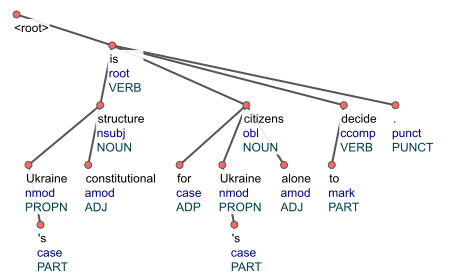
\includegraphics{img/cc-mark.png}
    \caption[Dependency Tree showcasing association of \texttt{PART} with \texttt{mark} deprel]{Dependency Tree for Example \ref{example:cc-mark} showcasing association of \texttt{PART} with \texttt{mark} deprel}
    \label{fig:func_multi}
\end{figure}

Furthermore, both the POS tags in question (\verb|SCONJ|, \verb|CCONJ|) can have other dependency relations attached to them as well. As such, it is difficult (and nonsensical) to limit the deprels for a particular POS tag to occur with a particular deprel (especially in this case). However, there might still be some processes we can observe (and correct). For example, if a particular token occurs more with the \verb|mark| deprel, but is consistently labelled as \verb|CCONJ|, the annotation should be taken a closer look at, and a possible disparity identified.

\section{\texttt{auxHead}: Auxiliary as Head of Dependency}
\label{future:auxHead}

In the discussion of this problem, we refer to the case when an auxiliary (marked by either of \verb|AUX| or \verb|aux|) is treated as the head of a dependency relation. Although allowed in certain cases, the auxiliary should not be marked as the dependency head in general sense. Consider the following example in Figure \ref{fig:aux-head-example}, taken directly from \cite{alzetta2017dangerous}. The token of interest is marked in bold.

\begin{example}
\textbf{ }\\
\textbf{Text (\texttt{it}):} Per noi \textbf{\`e} stato sufficiente che andassero via\\
\textbf{Lit.:} For us it-has been enough that they-went away\\
\end{example}
    
\begin{figure}[H]
    \centering
    \begin{subfigure}{.45\textwidth}
  \centering
  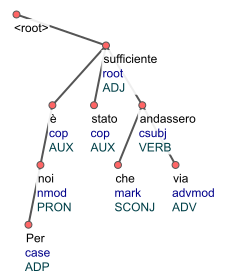
\includegraphics[scale=0.90]{img/before-aux.png}
  \caption{Original (Incorrect) Annotation}
  \label{fig:aux-head-skewed}
  \end{subfigure}
  \begin{subfigure}{.45\textwidth}
  \centering
  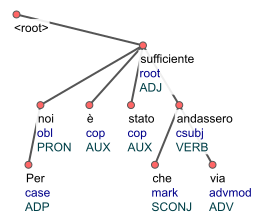
\includegraphics[scale=0.90]{img/after-aux.png}
  \caption{Corrected Annotation}
  \label{fig:aux-head-corrected}
  \end{subfigure}
    \caption[Example tree from \cite{alzetta2017dangerous} showcasing \texttt{auxHead} error type]{Example tree from \cite{alzetta2017dangerous} showcasing \texttt{auxHead} error type. In the original example, \textbf{noi} (us) was annotated as a dependent of both  \textbf{Per} (for), and \textbf{\`e} (has-been). Under UD representation, there can not be more than one head for any given node in regular annotation. As such, we believe it was a typo in the publication and not in their data. In this figure, we show the corrected dependencies.}
    \label{fig:aux-head-example}
\end{figure}
    
In the figure, notice how the originally incorrect annotation has \textit{\`e} (has-been) with POS \verb|AUX| serving as a dependency head. \citeauthor{alzetta2017dangerous} notice that this particular error, classified as a head identification error, contributes to around 13 \% of the total discovered erroneous instances. Since it is difficult to separate and identify the instances marked correctly as \verb|AUX| (cf. Chapter \ref{chap:failures} for the experiment on attempt at differentiation between \verb|AUX| and \verb|VERB|  tags), the attempt at the solution for this problem was not worked at.

\section{\texttt{nmod4obl}: Confusion of \texttt{nmod} and \texttt{obl} Relations}
\label{sec:probnmod4obl}

In UDv1, \verb|nmod| relation was used for nominals modifying either predicates or other nominals. Following a change in guidelines in v2, the deprel was restricted to modifying nominals. Furthermore, a new relation \verb|obl| (oblique) was introduced for oblique dependents of predicates.

To put it simply, this conversion implied the following in an equation format, where \(\verb|x|_{vi}\) refers to the dependency relation \(\verb|x|\) as used in version \(i\) of UD treebanks:

\begin{equation*}
    \boxed{\texttt{nmod}_{v1} = \texttt{nmod}_{v2} \cup \texttt{obl}}
\end{equation*}

Depending on the parent node, the relations were modified as follows:

\begin{enumerate}
    \item If the parent node was a verb, the deprel was changed from \texttt{nmod} to \texttt{obl}.
    \item If the parent was a nominal predicate, the deprel could be either of \texttt{nmod} or \texttt{obl}, depending on if only the nominal was being modified, or the whole clause was being modified.
    \item If the parent was a nominal, but not a nominal predicate, there was no change in the deprel.
    \item If the parent was an adjective or an adverb, the deprel would be changed to \texttt{obl}, based on additional conditions.
    \item In case none of the above conditions held true, the instance would deserve individual treatment.
\end{enumerate}

The change in definition from UDv1 to UDv2 was the primary cause of the error, as identified in \cite{alzetta2017dangerous}. In the same work, the authors note that this error contributes to around 7 \% of total discovered errors in the newspaper section of the Italian UD Treebank (IUDT). In the work, the authors attribute this error pattern to annotation inconsistency internal to the treebank. Although a significantly important error, this is not covered in the scope of the current research. Nonetheless, this is an important error that should be taken care of in future.

\section{Punctuation}

The UD Annotation guidelines on punctuation are simple and straightforward\footnote{\url{https://universaldependencies.org/u/overview/specific-syntax.html\#punctuation}}. There are discrepancies when it comes to implementation of the guidelines. Some of them are listed as below:

\begin{enumerate}
    \item It is difficult to identify the next conjunct in case of missing \verb|CCONJ| and \verb|SCONJ| tags as in case of asyndetic coordination. In such cases, the information about the next conjunct should be deduced semantically in most cases. We saw a similar case in Section \ref{sec:conj-sand} (Example \ref{examp:nonconj} and Figure \ref{fig:nonconj}) where the next conjunct is not clear, owing to other (more suitable) deprel(s) being used in place of \verb|conj| deprel.
    \item Re-attachment of a punctuation node is a problem that goes with the previous instance since it's not always clear at what level the punctuation must attach to.
    \item For paired and nested punctuation, different languages use different sets of nested punctuation pairs, specifically with respect to quotation marks. As such, the treatment of paired punctuation pairs needs to be handled in a language-specific manner.
\end{enumerate}

The \verb|fixpunct.py| block in Udapi-python \citep{udapi} tries to take care of significant number of edge cases in different UD treebanks. However, a more concrete solution is needed for the problems aforementioned.

\section{Unspecified Dependencies - \texttt{dep} deprel}

According to the UD definition of \verb|dep| deprel\footnote{\url{https://universaldependencies.org/u/dep/dep.html}}, the deprel is reserved for cases when a more precise relation cannot be found. This can be either owing to the sentence splitting in treebanks of some languages, or owing to the limitation in parsing software. Nonetheless, the relation should be avoided as much as possible.

Noticing that some treebanks follow sentence splits where the parts of sentences might be labelled as different sentences (as in the example of a list), the deprel in question is more liable to be used in such instances. However, looking at the data in UDv2.4, some languages have more than 1\% of the tokens marked with such relation (Examples being \verb|ko|, \verb|ur|, \verb|ja|-BCCWJ, \verb|it|-PoSTWITA, \verb|hi|-HDTB, \verb|gl|-CTG, \verb|cs|-PDT, among others). While these might be all true positives in other languages, a significantly higher count of \verb|dep| is more troublesome and is less likely to be all true positives in such cases.

An experiment can be performed on such instances where the data without any \verb|dep| deprel is used as a training set to parse the instances with the deprel in question and then the results verified. Nonetheless, the cases of tokens marked with deprel in question need to be reduced in some languages. As such, we leave it as a problem for future researchers to tackle.